\section{Experiments}

\subsection{Datasets}

The six used datasets are summaries in Table.~\ref{tbl:dataset}.
\emph{DIGITS} is a subset of the optical recognition of handwritten digits dataset~\cite{kaynak1995methods} of 8x8 grayscale images.
\emph{COIL20} \cite{nene1996} is a dataset of 32x32 grayscale pictures of 20 rotated objects.
\emph{FASHION\_1K} contains 1000 grayscale images of size 28x28, sampled from Fashion-MNIST\cite{xiao2017/online} clothing dataset.
The grayscale images from there above datasets are normalized and used directly in the DR methods.

\emph{FASHION\_MOBILENET} contains features extracted from a subset of Fashion Product images dataset.\footnote{https://www.kaggle.com/paramaggarwal/fashion-product-images-dataset}
The MobileNet\cite{} with pre-trained weights from ImageNet is used for feature extraction, a transfer learning technique that uses the representation of the learned network (trained on a large-scale image classification task) to extract meaningful features for new samples.
The last fully connected layer of the network is replaced by a global average pooling layer\cite{} to obtain the flatten output vector of 1280 dimensions.
To speed up the DR methods, PCA is then applied to take only 75 features.

\emph{5NEWS} contains the text of 5 groups selected from the 20 Newsgroups dataset which are converted to a matrix of token counts via TF-IDF method.
The count vectors are then fed into Latent Dirichlet Allocation (LDA) model to extract 15 hidden topics, which are 15 features used for DR methods.

The open NEURON\_1K~\cite{neuron1k} dataset contains 1301 Brain Cells from an E18 Mouse, processed and provided by 10X Genomics,
a company who provides chromium single cell gene expression solution and publics several genetic datasets.\footnote{https://www.10xgenomics.com/resources/datasets/, The datasets are licensed under the Creative Commons Attribution license.}
The processed data have 10 PCA features and labeled in 6 classes found by a graph-based clustering method.


\begin{table*}[width=\textwidth,cols=6,pos=h]
\caption{Description of six selected datasets with samples for the image datasets.}\label{tbl:dataset}
\begin{tabular}{m{3cm} m{4.8cm} m{8cm}}
\toprule
Dataset name & Samples & Description \\
\midrule

COIL20
    & 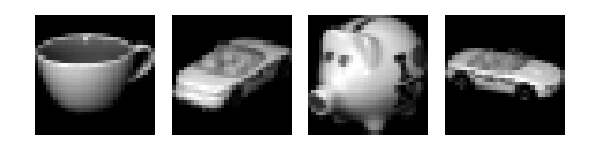
\includegraphics[width=\linewidth]{COIL20_samples}
    & 1440 grayscale images of size 32x32, belonging to 20 classes.
    The raw images of 1024 dimensions are used directly for the DR methods.\\

DIGITS
    & 
\includegraphics[width=\linewidth]{DIGITS_samples}
    & 1797 grayscale images of size 8x8 of 10 digits.
    The raw images of 64 dimensions are used directly for the DR methods.\\

FASHION\_1K
    & 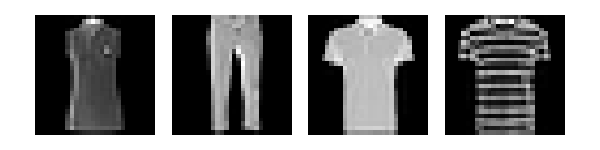
\includegraphics[width=\linewidth]{FASHION1000_samples}
    & 1000 grayscale images of size 28x28 of 10 classes, sampled from Fashion-MNIST dataset.
    The raw images of 768 dimensions are used directly for the DR methods.\\

FASHION\_MOBILENET
    & 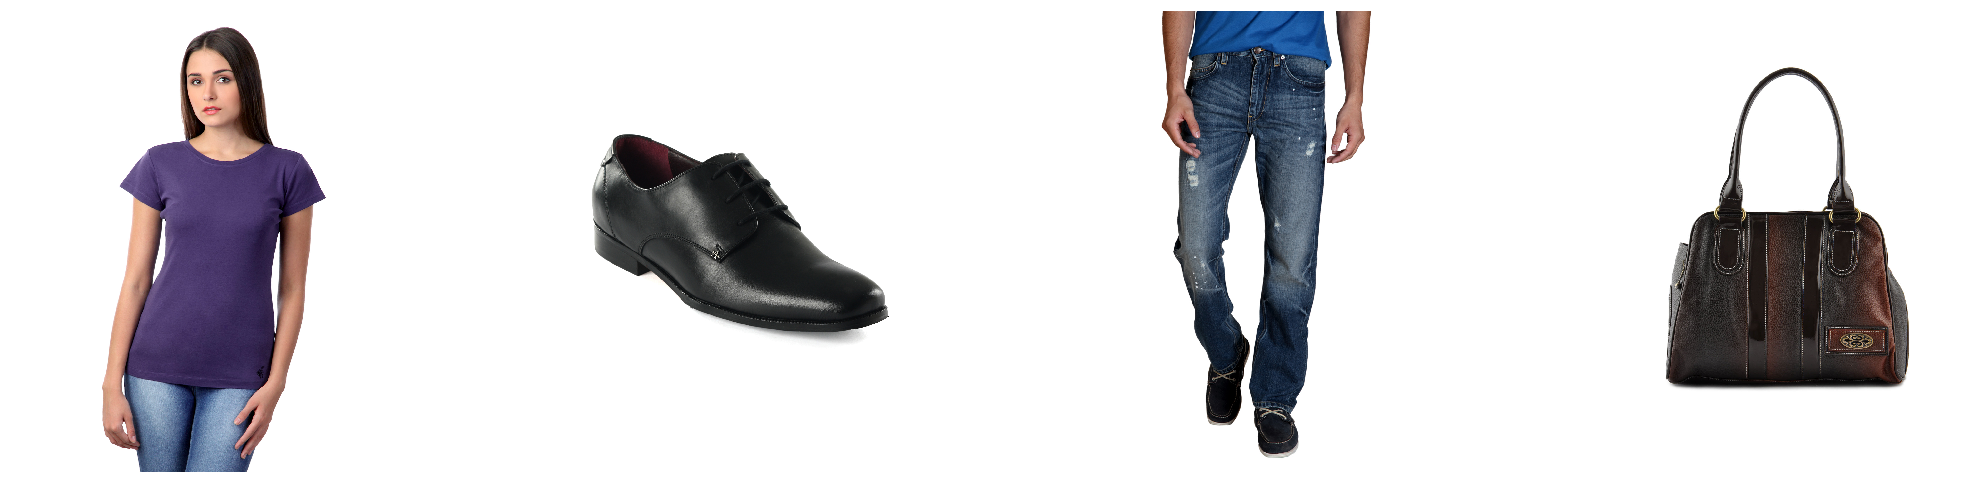
\includegraphics[width=\linewidth]{FASHION_PRODUCT_samples}
    & 1494 color images of various sizes belonging to 7 classes
    (\path{'Bags', 'Bottomwear', 'Jewellery', 'Sandal', 'Shoes', 'Topwear', 'Watches'}),
    sampled from Fashion Product images dataset.\\

5NEWS
    & 
\includegraphics[width=\linewidth]{20NEWS5_samples}
    & 5 groups of 2957 emails selected from 20Newsgroups dataset,
    including \path{'rec.autos', 'rec.sport.baseball','sci.crypt', 'sci.space', 'comp.sys.mac.hardware'}. \\

NEURON\_1K
    &
    & 1301 brain cells from a combined cortex, hippocampus and subventricular zone of an E18 mouse. \\

\bottomrule
\end{tabular}
\end{table*}





\subsection{Constraint Generation}


\subsection{Proof of Concept}
